\documentclass[11pt, a4paper, titlepage, twoside]{article}

\usepackage[utf8]{inputenc}
\usepackage[T2A, T1]{fontenc}
\usepackage[russian]{babel}

\renewcommand{\emph}{\textbf}
\usepackage{cmbright}

\usepackage[a4paper, left=3cm, right=3cm, top=3.5cm, bottom=3.5cm]{geometry}
\usepackage[automark, headsepline, footsepline]{scrpage2}
\usepackage{indentfirst}
\usepackage{graphicx}
\usepackage[labelfont=bf, textfont=it]{caption}
\usepackage{setspace}
\usepackage[nottoc]{tocbibind}

\newcommand{\version}{1.2.1}

\usepackage[
	pdftitle = {SortSimulation},
	pdfsubject = {Documentation},
	pdfauthor = {Peter\ {}Folta},
	pdfkeywords = {},
	pdfcreator = {},
	pdfproducer = {},
	colorlinks = true,
	linkcolor = black,
	anchorcolor = black,
	citecolor = black,
	filecolor = black,
	menucolor = black,
	pagecolor = black,
	urlcolor = blue]{hyperref}

\addto\captionsrussian{\renewcommand{\figurename}{Рис. №}}

\usepackage{listings}
\renewcommand{\lstlistingname}{Листинг №}
\renewcommand{\lstlistlistingname}{Листинги}
\lstset{basicstyle=\ttfamily, tabsize=4, numbers=left, numberstyle=\scriptsize, xleftmargin=20pt}

\title{СортСимулация}
\author{Peter Folta}

\clearscrheadfoot
\ihead[\headmark]{\headmark}
\ohead[\pagemark]{\pagemark}
\ifoot[SortSimulation~-- Документация]{SortSimulation~-- Документация}
\ofoot[Версия \version]{Версия \version}

\pagestyle{scrheadings}

\onehalfspacing

\begin{document}
	\pagenumbering{roman}
	
	\begin{titlepage}
		\begin{center}
			\vspace*{2.5cm}
			\Huge{\textbf{SortSimulation}}
			
			\vspace*{1.5cm}
			\LARGE{Документация}
			
			\Large{-- Русский --}
			
			\vspace*{3.75cm}
			\Large{Peter Folta}
		\end{center}
		
		\vspace*{8cm}
		\noindent{}Версия \version\newline{}
		Веб: \href{http://www.peterfolta.de/software/sortsimulation}{http://www.peterfolta.de/software/sortsimulation}\newline{}
		Авторские права 2008--2009 Peter Folta. Все права защищены.
	\end{titlepage}
	
	\setcounter{page}{2}
	
	\cleardoublepage{}
	\tableofcontents{}
	\newpage{}
	
	\pagenumbering{arabic}
	
	\section{Введение}
	
	SortSimulation является программой явы, которая изображает визуально разные способы сортировки. Это даст возможность с одной стороны лучше понять метод функции разных алгоритмов сортировки а на другой стороне поясняет разницы рабочего времени без сравнения лишь сухих чисел.
	
	\begin{figure}[h]
		\begin{center}
			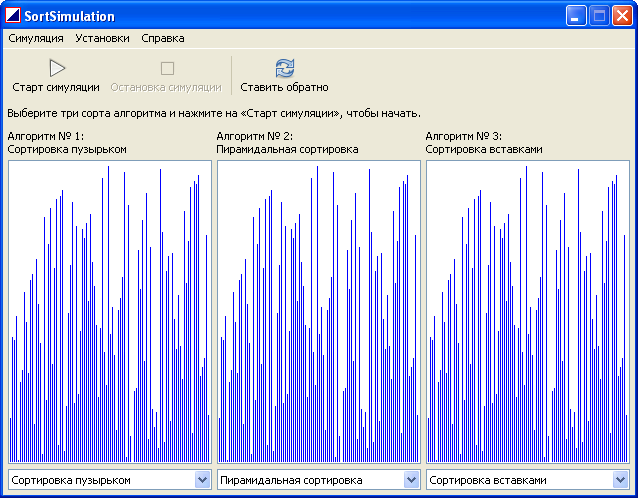
\includegraphics[scale=0.6]{images/image0.png}
			\caption{Центральное окно SortSimulation}
		\end{center}
	\end{figure}
	
	Эта документация содержает краткое введение и обслуживание SortSimulation и изображает затем поддерживающие способы сортировки включая имплементацию явы.
	
	\section{Обслуживание}
	
	Обслуживание SortSimulation возможно простое: Сразу после старта программы уже поля сортировки случайно наполнены. При этом в каждом из этих трёх полей та же самая исходная ситуация. После старта программы тоже установлены три разных способа сортировки; это можно видеть на ящиках выбора под полями сортировки.
	
	Чтобы сравнить друг с другом три алгоритма сортировки, выберите из ящиков выбора соответствующие способы. Симуляция начинается, когда щелкнете по \emph{Старт симуляции} на панеле инструментов, выберете соответствующее внесение в меню \emph{Симуляция} или щелкнете по ввод клавиша. Если хотите прорвать симуляцию, достаточно щелкнуть по Esc-клавиша или на кнопке \emph{Остановка симуляции}. Чтобы получить снова, после завершенной или прорванной симуляции, сдучайно наполнены поля, щелкните по \emph{Ставить обратно} или нажмите \texttt{Ctrl+N}.
	
	SortSimulation обнаруживает несколько установок, с которыми можете приноровить симуляцию. На этих установках остановимся подробно в следующем отрывке.
	
	\subsection{Установки}
	
	Для вас находятся в распоряжении разные установки, с которыми можете приноровить сортирующие симуляции в соответствии с вашим желанием. Эти возможности установок вы найдёте в меню \emph{Установки}:
	
	\begin{figure}[h]
		\begin{center}
			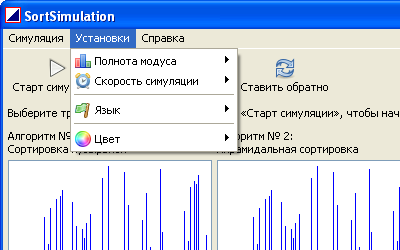
\includegraphics[scale=0.6]{images/image1.png}
			\caption{Меню «Установки»}
		\end{center}
	\end{figure}
	
	При помощи \emph{Полнота модуса} можете определить, каким способом должны быть наполнены поля сортировки, когда акция \emph{Ставить обратно} исполнена. При этом есть два модуса в распоряжении: случайный  (установлен; \texttt{Ctrl+R}) и инверс (\texttt{Ctrl+I}). В модусе \emph{Случайный} будут элементы при каждом новом наполнении полей случайно установлены. Так можно производить реалистическим способом опыт разных сортировок с не сортированными данными.
	
	В модусе \emph{Инверс} поля уже сортированно наполнены~-- разумеется наоборот (понижаемо а не повышаемо). Этой установкой можно видеть, как эффектно сортируют сортировки наполнены наоборот.
	
	Низшее меню \emph{Скорость симуляции} даст вам возможность приноровить скорость симуляции. У вас есть выбор из пятеро степеней. Так как например у алгоритма сортировка пузырьком, которая очень медленная, напрашивается высокая степень скорости симуляции, так стоит наблюдать например быструю сортировку на медленной степени скорости, чтобы лучше понять образ действия этого способа. Отдельные степени скорости можно получить на клавиши при помощи \texttt{Ctrl+Shift+(1-5)}.
	
	SortSimulation не пишет или не изменяет данные на вашем компьютере, поэтому программа начинается каждый раз с английским интерфейсом пользователя. Вы можете изменить язык в меню \emph{Язык} (англ.: \emph{Settings} > \emph{Language}).
	
	В последнем низшем меню \emph{Цвет} можно установить цвет балок. По стандарту установлен синий цвет. На выбор есть восемь различных цветов.
	
	\section{Алгоритм сортировки}
	
	\subsection{Сортировка пузырьком}
	
	Сортировка пузырьком является простым алгоритмом, которая сортирует элементы через \emph{постепенное сравнение}. Потому что сортировка пузырьком не эффектная, употребляется этот алгоритм часто как демонстрация плохого метода сортировки.
	
	\subsubsection{Идея сортировки пузырьком}
	
	Сортировка пузырьком сравняет два соседних элемента и обменяет их, если они находятся в неправильной последовательности. Этот процесс повторяется так долго, пока все элементы не стоят на правильном месте и так они сортируются.
	
	\subsubsection{Имплементация явы}
	
	\lstinputlisting[caption={Имплементация сортировки пузырьком}, label=lst:bubblesort, captionpos=b]{../Listings/Bubblesort.java}
	
	\subsection{Пирамидальная сортировка}
	
	Пирамидальная сортировка быстрый способ сортировки, который был развит в 1964 году \emph{Робертом В Флоудом} (англ. Robert W Floyd) и \emph{Й.\,{}В.\,{}Й. Вильямсом} (англ. J.\,W.\,J. Williams). Пирамидальная сортировка улучшение алгоритма \emph{сортировки выбором}.
	
	\subsubsection{Идея пирамидальной сортировки}
	
	Пирамидальная сортировка употребляет для сортировки специальную структуру данных: \emph{пирамиду}. Эта структура данных базирует на (почти) полном \emph{бинарном дереве}. Бинарное дерево является (почти) полным, когда все области, быть может без последней, полные.
	
	Когда сортированная очерёдность есть пирамидой, тогда можно взять и выдать самый большой элемент из \emph{корня дерева}. Чтобы прийти к следующему большому элементу, должна быть пирамида \emph{заново установлена}.
	
	\subsubsection{Имплементация явы}
	
	\lstinputlisting[caption={Имплементация пирамидальной сортировки}, label=lst:heapsort, captionpos=b]{../Listings/Heapsort.java}
	
	\subsection{Сортировка вставками}
	
	Сортировка вставками является простым методом сортировки. Она не так эффектна как другие комплексные алгоритмы, но её можно \emph{просто имплементировать} и она требует только короткое рабочее время при небольших или уже заранее сортированных данных.
	
	\subsubsection{Идея сортировки вставками}
	
	При сортировке вставками берётся один элемент из несортированной массы и вставляется на правильное место в расход последствия. Если последствие ещё пустое, элемент будет вставлен на первую позицию.
	
	Сортировка вставками не эффектна, потому что при ней надо часто передвигать элементы через дальнее расстояние.
	
	\subsubsection{Имплементация явы}
	
	\lstinputlisting[caption={Имплементация сортировки вставками}, label=lst:insertionsort, captionpos=b]{../Listings/Insertionsort.java}
	
	\subsection{Сортировка слиянием}
	
	Сортировка слиянием является рекурсным и стабильным сортировным алгоритмом, который базирует как и \emph{быстрая сортировка} на принципе \emph{разделяй и властвуй}. Сортировка слиянием была представлена в 1945 году \emph{Джоном фон Нейманом} (англ. John von Neumann).
	
	\subsubsection{Идея сортировки слиянием}
	
	Сортировка слиянием разбирает последствие, которое должно быть сортировано, на несколько малых последствий, каждая из них будет сортирована для себя. Затем будут эти сортированные малые последствия собраны методом молнии в большое последствие, пока все элементы не сортированные.
	
	\subsubsection{Имплементация явы}
	
	\lstinputlisting[caption={Имплементация сортировки слиянием}, label=lst:mergesort, captionpos=b]{../Listings/Mergesort.java}
	
	\subsection{Быстрая сортировка}
	
	Быстрая сортировка \emph{самый быстрый способ сортировки}, который базирует на принципе \emph{разделяй и властвуй}. Этот рекурсный алгоритм быстрой сортировки развил в своей первоначальной формулировке \emph{Ч. Энтони Р. Хоар} (англ. C.\,{}A.\,{}R. Hoare) в 1960 году.
	
	\subsubsection{Идея быстрой сортировки}
	
	Последствие, которое должно быть сортированным, с начала разделяется так на две части, что все элементы в первой части менее или равны всем элементам второй части (\emph{разделяй}). Затем сортируются рекурсно эти две части независимо друг от друга этим же самым способом (\emph{властвуй}). В последнем шагу составляют эти две части сортированное последствие (\emph{соединяй}).
	
	Это разделение реализуется при помощи одного \emph{опорного элемента}, который выбирается в первом шагу из последствия. Все элементы последствия, которые \emph{меньше} опорного эдемента, придут в первю часть. Все елементы, которюе \emph{больше} опорного елемента придут во вторую часть. У элементов, которые одинаковы с опорным элементом, всё ровно, до которой части они придут.
	
	\subsubsection{Имплементация явы}
	
	\lstinputlisting[caption={Имплементация быстрой сортировки}, label=lst:quicksort, captionpos=b]{../Listings/Quicksort.java}
	
	\subsection{Сортировка выбором}
	
	Сортировка выбором является наивным сортировным алгоритмом, который работает на месте. Эту сортировку можно сравнить с сортировкой вставками.
	
	\subsubsection{Идея сортировки выбором}
	
	Сортировка выбором разделяет последствие, которое должно быть сортировано, на \emph{сортированную} и \emph{несортированную} части. Сортированная часть в начале пустая. Сортировка выбором ищет самый малый элемент в несортированной части последствия и сменяет его на первый элемент. После этого шага последствие сортировано до этой позиции. Сортированная часть становится так больше на один элемент, несортированная часть на один элемент меньше. Этот метод повторяется, пока целое последствие не сортировано.
	
	\subsubsection{Имплементация явы}
	
	\lstinputlisting[caption={Имплементация сортировки выбором}, label=lst:selectionsort, captionpos=b]{../Listings/Selectionsort.java}
	
	\subsection{Сортировка Шелла}
	
	Сортировка Шелла метод сортировки, который базирует на \emph{сортировке вставками}. Сортировка Шелла была развита в 1959 году \emph{Доналдом Л. Шеллом} (англ. Donald L. Shell).
	
	\subsubsection{Идея сортировки Шелла}
	
	Сортировка Шелла компенсирует недостаток сортировки вставками, при которой надо элементы передвигать через дальнее растояние. Сортировка Шелла производит к тому одну \emph{к-раскалывающуюся матрицу}, которой столбцы отдельно сортируются. После этих шагов уже последствие грубо сортировано. Этот шаг повторяется, причём количество столбцов уменьшается при каждом выполнении, пока матрица не состоит только из одного отдельного столбца.
	
	\subsubsection{Имплементация явы}
	
	\lstinputlisting[caption={Имплементация сортировки Шелла}, label=lst:shellsort, captionpos=b]{../Listings/Shellsort.java}
	
	\section{Сотрудники}
	
	Здесь надо выразить благодарность следующим персонам, которые деятельно оказали помощь развитию SortSimulation. Новые сотрудники (переводчики, чертёжники, составители документаций и так далее) ищутся постоянно~-- если вы интересуетесь, войдите в контакт с Петром Фолта (нем. Peter Folta).
	
	\subsection{Переводчики}
	
	\begin{itemize}
		\singlespacing
		\item{Folta, Lucia Sonja~-- Русский}
		\item{Folta, Peter~-- Английский, Немецкий}
		\item{Müllner, Jan Sebastian~-- Французский, Испанский}
	\end{itemize}
	
	\section{Контакт}
	
	\noindent{}Peter Folta\newline{}
	Humboldtstrasse 9\newline{}
	34497 Корбах (нем. Korbach)\newline{}
	Германия\newline{}
	
	\noindent{}\textbf{E-Mail:} \href{mailto:mail@peterfolta.de}{mail@peterfolta.de}\newline{}
	\textbf{Веб:} \href{http://www.peterfolta.de/}{http://www.peterfolta.de/}
	
	\begin{thebibliography}{99}
		\bibitem{Lang}
			\textsc{Lang}, Prof. Dr. Hans Werner: \emph{Algorithmen in Java}. 2-е издание 2006 г. Мюнхен: Oldenbourg Wissenschaftsverlag GmbH 2006. ISBN 978-3-486-57938-3, стр.~5--52
		\end{thebibliography}
	
	\listoffigures{}
	\lstlistoflistings{}
	\addcontentsline{toc}{section}{Листинги}
\end{document}